\documentclass{article}
\usepackage{mathtools, blkarray}
\usepackage{graphics,graphicx}
\usepackage{tikz}

\usetikzlibrary{arrows,snakes,backgrounds}



\makeatletter
% we use \prefix@<level> only if it is defined
\renewcommand{\@seccntformat}[1]{%
  \ifcsname prefix@#1\endcsname
    \csname prefix@#1\endcsname
  \else
    \csname the#1\endcsname\quad
  \fi}
% define \prefix@subsection
\newcommand\prefix@subsection{}
\makeatother

\makeatletter
% we use \prefix@<level> only if it is defined
\renewcommand{\@seccntformat}[1]{%
  \ifcsname prefix@#1\endcsname
    \csname prefix@#1\endcsname
  \else
    \csname the#1\endcsname\quad
  \fi}
% define \prefix@subsubsection
\newcommand\prefix@subsubsection{ }
\makeatother

\newcommand{\mytilde}{\raise.17ex\hbox{$\scriptstyle\mathtt{\sim}$}}


\begin{document}

\title{Math 775: Homework 2}
\author{Alex Dewey}


\maketitle


\section{Exercises}

\subsection{Exercise 1.}

\subsubsection{i.}

\[P(y\vert\theta) = {y + r - 1 \choose y}\theta^r(1 - \theta)^y, y= 0, 1, ...\]
\[\log P(y\vert\theta) = \log {y + r - 1 \choose y} + r\log\theta + y\log(1 - \theta)\]
\[{\delta\log P(y\vert\theta) \over \delta\theta} = {r \over \theta} - {y \over 1 - \theta}\]
\[{\delta^2\log P(y\vert\theta) \over \delta\theta^2} = -{r \over \theta^2} - {y \over (1 - \theta)^2}\]

r is a given constant and \(E(y \vert \theta)\) is just the expectation of a negative binomial distribution
\(E(y \vert \theta) = {r\theta \over 1 - \theta}\) (we can derive this by using the infinite sum 
\[\theta + \theta^2 +... = {\theta \over 1 - \theta}\] for r = 1 and treating the spaces between
 negative trials as r IID draws).

Anyway, the Fisher information follows from this:

\[J^{\text{Fisher}}(\theta) = -E \big[ {\delta^2\log P(y\vert\theta) \over \delta\theta^2} \big \vert \theta \big]
= {r \over \theta^2} + {{r\theta \over 1 - \theta} \over (1 - \theta)^2} = {r \over \theta^2} + {r\theta \over  (1 - \theta)^3}\]

\subsubsection{ii.}

\[P(y\vert\theta) = {1 \over y!} \theta^y e^{-\theta} \]

\[\log P(y\vert\theta) = -\log{y!} + y\log\theta - \theta \]

\[{\delta\log P(y\vert\theta) \over \delta\theta} = {y \over \theta} - 1 \]

\[{\delta^2\log P(y\vert\theta) \over \delta\theta^2} = -{y \over \theta^2}\]

Now, the expectation of y given \(\theta\) is \(\theta\), because by definition
y is a Poisson distribution with mean \(\theta\). So we have:

\[J^{\text{Fisher}}(\theta) = -E \big[ {\delta^2\log P(y\vert\theta) \over \delta\theta^2} \big \vert \theta \big]
= -E(-{y \over \theta^2} | \theta) = {\theta \over \theta^2} = {1 \over \theta}\]

\subsubsection{iii.}

Since \(\sigma^2\) is known, we can use the standard normal density:

\[P(y\vert\mu) = {1 \over \sqrt{2\pi}\sigma}e^{-{1 \over 2\sigma^2}(y - \mu)^2}\].

\[\log P(y\vert\mu) = \log{1 \over \sqrt{2\pi}\sigma} - {1 \over 2\sigma^2}(y - \mu)^2\]

\[{\delta\log P(y\vert\mu) \over \delta\mu} = {1 \over \sigma^2}(y - \mu)\]

\[{\delta^2\log P(y\vert\mu) \over \delta\mu^2} = -{1 \over \sigma^2}\]

So \[J^{\text{Fisher}}(\mu) = E({1 \over \sigma^2} \vert \mu) = {1 \over \sigma^2}\]

So the Fisher information is the constant, known value \(1 / \sigma^2\).

\subsubsection{iv.}

By \textit{Bayesian Data Analysis} (Gelman, pg. 43), we can write the likelihood for a normal model with known mean \(\mu\)
and unknown variance \(\sigma^2\) (with y an iid vector of n observations) as:

\[p(y \vert \sigma^2) \propto \sigma^{-n} e^{-{n \over 2\sigma^2}v}\]

with \[v = {1 \over n} \sum_i^n (y_i - \mu)^2\].

\[p(y \vert \sigma^2) = C (\sigma^2)^{-n / 2} e^{-{nv/ 2\sigma^2}}\]

\[\log P(y\vert\sigma^2) = \log C + -{n \over 2}\log{\sigma^2} + -{nv \over 2\sigma^2}\]

\[{\delta\log P(y\vert\sigma^2) \over \delta\sigma^2} = -{n \over 2\sigma^2} + {nv \over 2(\sigma^2)^2}\]

\[{\delta^2\log P(y\vert\mu) \over \delta(\sigma^2)^2} =  {n \over 2(\sigma^2)^2} - {nv \over (\sigma^2)^3}\]

\((nv \vert \sigma^2) \mytilde \sigma^2\chi^2_{n} \) and \(E( \sigma^2\chi^2_{n}) = n\sigma^2\) by definition (note that 
\(v\) is centered around the population mean \(\mu\), not around the sample mean of y, so we have n degrees of freedom). So:

\[J^{\text{Fisher}}(\mu) = 
-{n \over 2(\sigma^2)^2} + {n\sigma^2 \over (\sigma^2)^3} = {n \over 2(\sigma^2)^2}\].

\newpage

\subsection{Exercise 2.}

Suppose \(p(y \vert \theta) \mytilde Bin(n = 50, \theta)\) where 
\(p(\theta) = 0.5 \times Beta(10, 20) + 0.2 \times Beta(15,15) + 0.3 \times Beta(20,10)\)

We want to compute and then plot \(p(\theta \vert y=14)\).

First thing to note is that we don't have to integrate anything
to get the answer. The binomial distribution is just
the result of n iid (hence exchangeable) Bernoulli trials, and
the beta distribution is a conjugate prior with respect to
exchangeable Bernoulli data.

Therefore, once we know the prior and data, we can immediately get a posterior
for each of the distributions. And we can treat each beta distribution in \(\theta\) separately 
(since integration over our Prior \(\times\) Likelihood is linear).

So we can simply add y=14 successes and 36 failures to each of our 
beta distributions to get the form 

\(p(\theta \vert y = 14) = 0.5 \times Beta(24, 56) + 0.2 \times Beta(29, 51) + 0.3 \times Beta (34, 46)\).

\begin{figure}[!ht]
  \caption{The posterior and prior in Question 2.}
  \centering
    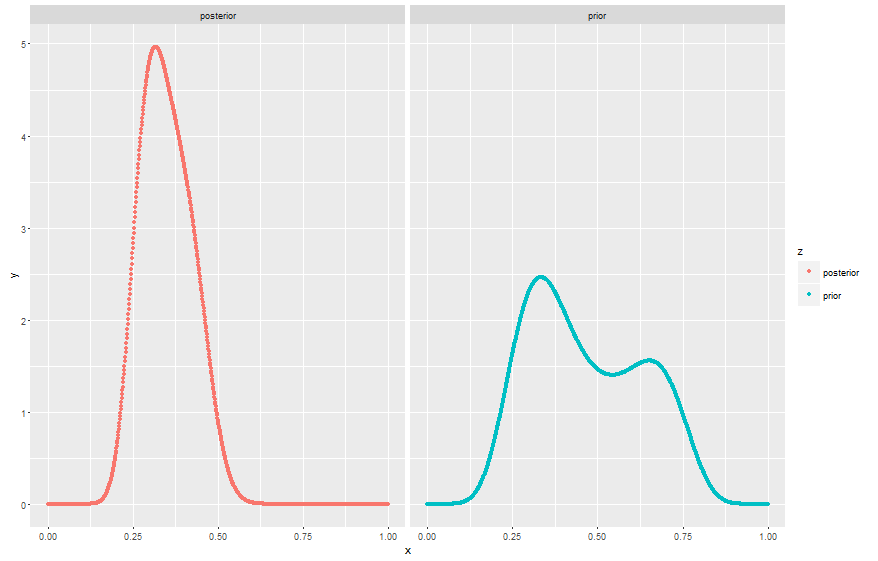
\includegraphics[width=\textwidth]{Question2}
\end{figure}

\newpage

\subsection{Exercise 3.}

Because the W and B follow independent Poisson 
distributions, we can just multiply \(\text{Poisson}(\lambda + \mu)\) and 
\(\text{Poisson}(\lambda)\) in order to get the likelihood. The
derivations are straightforward and 
the functions I used for each observed value of \((W, B)\) are below.

\[p(W=5, B=2 \vert \Theta = (\mu, \lambda)) = 
{1 \over 5!2!} (\mu + \lambda)^5 {\lambda}^2 e^{-(\mu + 2\lambda)} \]
\[p(W=3, B=4 \vert \Theta = (\mu, \lambda)) = 
{1 \over 3!4!} (\mu + \lambda)^3 {\lambda}^4 e^{-(\mu + 2\lambda)} \]

The contour plots are below. The first plot shows that the maximum likelihood value
for \((W=5, B=2)\) is \(\Theta = (\mu = 3, \lambda = 2)\).

This fits with intuition, since W is distributed with mean
\(\mu + \lambda\) and B is distributed with mean \(\lambda\).

For \((W=3, B=4)\), the situation is more complicated.
The likelihood appears to take
on a maximum outside our domain, at \(\Theta = (\mu = -1, \lambda = 4)\).
Because these are meant to be signals which have, by construction, \(\mu, \lambda \geq 0\),
we can't draw from \(\mu = -1\). But it's clear that the signals would hit a maximum
likelihood there if we could draw from it.


\begin{figure}[!ht]
  \caption{The two contour plots.}
  \centering
    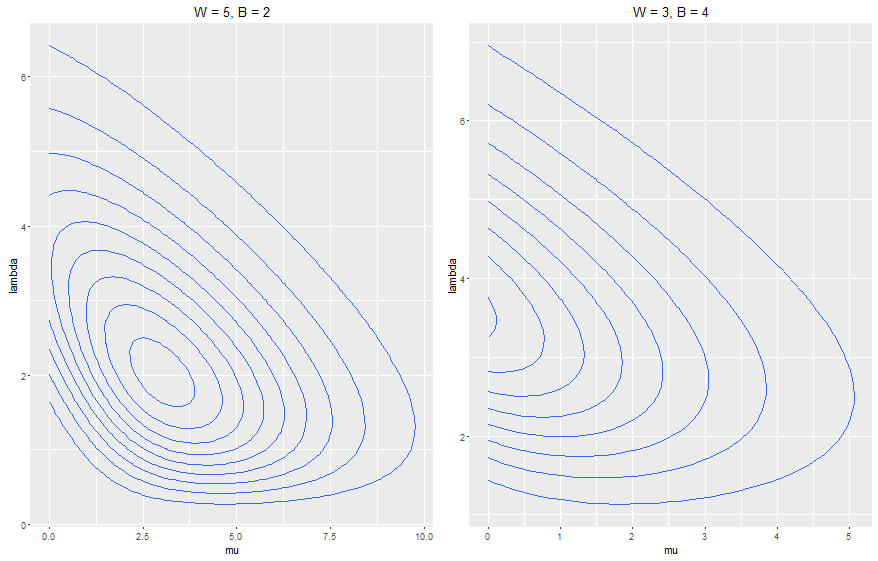
\includegraphics[width=\textwidth]{Question3}
\end{figure}

\newpage

\subsection{Exercise 4.}

For \((y_1, y_2)\), there is only one non-trivial case in which
permuting the indices \(p(y_1, y_2)\) is even possible.

In particular, the exchangeability condition holds if and only if
\(p(1, 0) = p(0, 1)\). For this distribution, that is clearly true.

\begin{equation}
p(y) = \int_0^1  \theta^{\sum y_i}(1 - \theta)^{2 - \sum y_i} p(\theta) \delta\theta
\end{equation}

To get equation (1), we would need the following four conditions to hold:

\[p(0,0) = \int_0^1   (1 - \theta)^{2} p(\theta) \delta\theta = 0\]
\[p(0,1) = \int_0^1 \theta^1(1 - \theta)^1 p(\theta)\delta\theta = 0.5\]
\[p(1,0) = \int_0^1 \theta^1(1 - \theta)^{1} p(\theta)\delta\theta = 0.5\]
\[p(1,1) = \int_0^1 \theta^{2} p(\theta)\delta\theta = 0 \]

Note that in the first and fourth equations, \(\theta^2 > 0\) and \((1 - \theta)^2 > 0\)
for all values of \(\theta\) in the interior of the interval [0,1]. 

Without writing out the Riemann sums for the first and fourth integrals,
it's clear that if we require our prior \(p(\theta) \geq 0\) 
to be a probability distribution, 
then we must have \(p(\theta) = 0\) for all but a subset of measure zero
over \([0, 1]\).

Therefore the second and third equations,
which are being multipled by the same \(p(\theta)\), over
the same subset, must also integrate to zero. But they don't, so 
such a \(p(\theta)\) cannot exist. So the condition analogous
to De Finetti's Theorem cannot hold for this distribution.

\subsection{Exercise 5.}

\subsubsection{a.}

When \(\alpha = \beta = 1\), the beta prior \(B(\alpha, \beta)\) is uniform. So it's natural to take this
as the form of the prior and incorporate the data \(\hat{\theta} = y / n\) as n Bernoulli trials.

\(p(y=k \vert \theta) = {n \choose k} \theta^{k}(1 - \theta)^{n-k} = {\Gamma(n + 1) \over \Gamma(k + 1) \Gamma(n - k +1)} \theta^{k}(1 - \theta)^{n-k} \).

Integrating this function over \(\theta\), we note that it's a beta distribution with parameters \(n + 1, k + 1\) (which integrates to 1) 
but multiplied by \({\Gamma(n + 1) \over \Gamma (n + 2)} = {1 \over n + 1}\).

So  our predictive prior is \(p(y = k) = {1 \over n + 1}\) for all k.

\subsubsection{b.}

The posterior distribution is 
\(\text{Beta}(\alpha + k, \beta + (n - k))\) with mean \[\alpha + y \over \alpha + \beta + n\].

We can rewrite this posterior mean as a weighted average of the prior mean and the sample mean:

\[{\alpha + y \over \alpha + \beta + n} = {y \over n}{n \over \alpha + \beta + n} + {\alpha \over \alpha + \beta}{\alpha + \beta \over \alpha + \beta + n}\].

Since, by definition, we have \(\alpha, \beta, y, n \geq 0\) and \({\alpha + \beta \over \alpha + \beta + n} + {n \over \alpha + \beta + n} = 1\),
the weighed average above is a convex sum and it must lie between the prior and the sample means.

\subsubsection{c.}

The variance of Beta(1,1) (our uniform prior) for \(\theta\) is \[{\alpha\beta \over (\alpha + \beta)^2(\alpha + \beta + 1)} = {1 \over 2^2 * 3} = 1/12\].

The variance of our posterior distribution \(p(\theta \vert y = k) = \text{Beta}(1 + k, 1 + (n - k))\) is

\[{\alpha\beta \over (\alpha + \beta)^2(\alpha + \beta + 1)} = {(1 + k) (1 + (n - k)) \over (n+2)^2 (n+3)}\].

The numerator is the only part that depends on k, and (if we allow any real k),
it attains a maximum at \(k = n/2\) by a 
standard argument (suppose not: then we could write it as \( ((1 + n/2) + a)((1 + n/2) - a) = (1 + n/2)^2 - a^2\)
for some \(a > 0\). Then we would have \(a^2 \leq 0\), a contradiction). So we want to show that

\({(n/2 + 1)^2 / (n + 2)^2 (n+3)} > 1/12\) for any \(n > 0\). Note that \( 2(n/2 + 1) = (n + 2)\), so this
reduces to \({1 \over 4(n+3)} < {1 \over 12}\).

So the posterior variance must be less for any observed data than that of the uniform prior.

\subsubsection{d.}

Start with a prior of Beta(20, 1), \(n = 19, k=0\). So our posterior ends up as Beta(20,20).

The variance of our prior is \({20 \over 21^2 * 22} \approx 0.00206\). The variance of our
posterior is \({400 \over 40^2*41} \approx 0.00610\), or nearly 3 times higher.


\subsection{Exercise 8}

By Gelman (pg. 42), the posterior is just \(N(\theta \vert \mu_n, \tau_n^2)\)
with \[\mu_n = {{{1 \over \tau_0^2}\mu_0 + {n \over \sigma_0^2}\bar{y}} \over { {1 \over \tau_0^2} + {n \over \sigma^2}}}\]
and \[{ 1 \over \tau^2_n} = {{1 \over \tau_0^2} + {n \over \sigma^2}}\],
with prior \(N(\mu_0, \tau_0^2)\) and observed y and known \(\sigma^2\).

\subsubsection{a.}

We have \(\bar{y} = 150, \sigma^2 = 20^2, \mu_0 = 180, \tau_0 = 40\).

So our posterior distribution is \(N(\theta \vert \mu_n, \tau_n^2)\)
with:

\[{ 1 \over \tau^2_n}= {{1 \over 1600} + {n \over 400}}\] and 
\[\mu_n = {{{180 \over 1600} + {150 \over 400}} \over {{1 \over 1600} + {n \over 400}}}\]


\subsubsection{b.}

The predictive posterior distribution for \(\tilde{y}\) is a normal distribution
with  \(N(\theta \vert \mu_n, \tau_n^2 + \sigma^2)\), where \(\mu_n, \tau_n\) are
defined as in part (a.). We get extra variance from the fact that we're
predicting a single observation rather than the underlying parameter \(\theta\).




\subsubsection{c-d.}

For the posterior and posterior predictive intervals, I used R to implement the above discussion (using \(\mu_n \pm 1.960*\tau_n\) for
\(\theta\) and \(\mu_n \pm 1.960*\sqrt{\tau_n^2 + \sigma^2}\)) for \(\tilde{y}\)).

The results I found were:

\begin{tabular} {| r | c | c |}
\hline
Interval &\(n = 10\)&\(n = 100\)\\ \hline
\(\theta\) &(138.488, 162.976) & (146.160, 153.990)\\ \hline
\(\tilde{y}\) &(109.664, 191.799)&(110.680, 189.470)\\ \hline
\end{tabular} 

\newpage

\subsection{Exercise 10}

\subsubsection{a.}

The first thing to note is that for \(n < 203\), we must have \(p(y = 203 \vert N=n) = 0\).

For \(n \geq 203\), we're dealing with a uniform likelihood. \(p(y = 203 \vert N=n) = {1 \over n}\).

So the posterior distribution is
\(p(N=n \vert y = 203) \propto {1 \over n}({99 \over 100})^n\) for \(n \geq 203\), where constants
have been removed.

\subsubsection{b.}

Analytically (after summing from 203 to 50000 to get the normalizing constant),
 I got a mean of 279.088 and a standard deviation of 79.96.

\subsubsection{c.}

I tried the Poisson non-informative prior \(\sqrt{1 \over \lambda}\) with \(\lambda = 0.01\).

The mean didn't converge as I increased \(n\),
because the normalizing constant is given by the harmonic series from 203 to n,
and this series diverges. Therefore, the mean and standard deviation
continued to increase with \(n\).

\end{document}